%! Author = weile
%! Date = 13.02.2025

% Preamble
\documentclass{article}

% Packages
\usepackage{amsmath}
\usepackage{csquotes}
\usepackage{listings}
\usepackage{graphicx}

\title{Anleitung zum Gebrauch der EnergyApp}

\author{
    Weilert Alexander, 12119653
    \and
    Kühnel Philipp,
}

\maketitle

% Document
\begin{document}
    \section{Abstract}
    Dieses Dokument beschreibt eine Anleitung zur Implementierung der EnergyApp, die wir im Rahmen der
    Lehrveranstaltung \enquote{Software Praktikum} entwickelt haben.
    Ziel ist es, die wesentlichen Konzepte und technischen Details der Implementierung zu erläutern.

    \section{Main.dart}
    In der Datei \enquote{Main.dart} wird die App initialisiert.
    Basierend auf einem Gedächtnisprotokoll wurde versucht, die ursprüngliche Implementierung so genau wie möglich nachzubilden.
    Daher wird in dieser Dokumentation nur ein kleiner Teil davon ausführlicher erklärt.
\begin{lstlisting}[language=Dart]
void main() async {
    WidgetsFlutterBinding.ensureInitialized();
    final database = PostgresDatabase();
    await database.connectToDatabase().timeout(Duration(seconds: 20));
    runApp(MyApp(database: database));
    //...
}
class MainScreen extends StatelessWidget {
  final PostgresDatabase database;

  MainScreen({required this.database});
    //...
}
\end{lstlisting}
    \\
    Im obigen Codeausschnitt führen wir zunächst eine Initialisierung der Datenbankverbindung durch.
    Dies stellt sicher, dass eine stabile Verbindung zur Datenbank besteht, sodass spätere
    Datenabfragen effizient erfolgen können. \\
    Die Method \enquote{connectToDatabase()} wird mit einem Timeout von 20 Sekunden aufgerufen.
    Sollte die Verbindung innerhalb dieser Zeit nicht erfolgreich hergestellt werden,
    bricht der Verbindungsaufbau ab. \\
    Die Funktion \enquote{WidgetsFlutterBinding.ensureInitialized()} wird am Anfang der \enquote{main()} Methode
    aufgerufen, um sicherzustellen, dass Widgets korrekt initialisiert werden können, insbesondere bei der
    Verwendung von asynchronen Operationen wie der Datenbankverbindung.
    \begin{lstlisting}[language=Dart]
Future<void> connectToDatabase() async {
  try {
    connection = PostgreSQLConnection(
      "10.0.2.2",   //"192.168.56.1",
      5432,
      "postgres",
      username: "postgres",
      password: "alex",
    );
    await connection.open();
    print("Verbindung wurde erfolgreich hergestellt.");
  } catch (e) {
    print('Fehler beim Herstellen der Verbindung zur Datenbank: $e');
  }
}
    \end{lstlisting}
    Ein Großteil der Probleme, auf die wir gestoßen sind, war auf diesen kleinen Codeausschnitt zurückzuführen,
    genauer gesagt auf die verwendete IP-Adresse. \\
    In einer Testumgebung bzw.\ einem Emulator, wie wir ihn verwendet haben, besitzt das virtuelle Gerät eine eigene
    IP-Adresse, über die eine Verbindung zur Datenbank hergestellt werden kann.
    Bei Android-Emulatoren ist \enquote{10.0.2.2} eine spezielle Adresse, die als Alias für den Hostrechner dient.
    In einem produktiven System würde man stattdessen \enquote{localhost} oder \enquote{192.168.56.1} verwenden,
    je nach Netzwerkkonfiguration. \\
    Nach der IP-Adresse folgt der Port, der für PostgreSQL standardmäßig \enquote{5432} ist.
    Danach werden der Datenbankname, der Benutzername und das Passwort angegeben, welche individuell an die eigene
    Umgebung angepasst werden müssen. \\
    Da die Datenbankverbindung asynchron hergestellt wird, läuft der Verbindungsaufbau im Hintergrund weiter, während
    bereits das Frontend der Anwendung gerendert wird.
    Dies verbessert die Benutzererfahrung, da die App nicht blockiert wird, falls die Verbindung zur Datenbank einige
    Sekunden in Anspruch nimmt.
    \begin{figure}
        \centering
        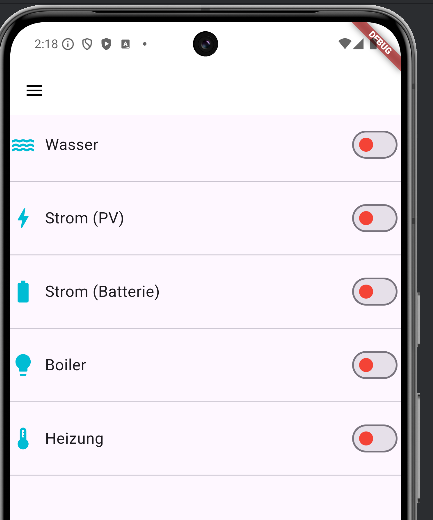
\includegraphics[height=4cm]{images/FrontEndScreenshot}
        \caption{Frontend der EnergyApp mit grundlegenden Funktionen}
    \end{figure}
    Das Menü wird über einen sogenannten \enquote{AppDrawer} realisiert, der sich oben links befindet und
    durch eine Berührung aufgerufen werden kann.
    Dieser Drawer wurde mit Hilfe von ChatGPT entwickelt und bietet Zugriff auf weitere Funktionen der Anwendung. \\
    Ein Klick auf \enquote{Wasser} hat derzeit keine Funktion, da dieser Button als Dummy-Funktion dient. \\
    Hingegen führen Klicks auf \enquote{Boiler} oder \enquote{Heizung} dazu, dass mithilfe der Funktion
    \enquote{MaterialPageRoute} eine Navigation in die nächste Ansicht erfolgt.
    Dabei wird eine neue Seite geladen, die die Graphen aufruft.
    Eine detaillierte Beschreibung folgt in einem späteren Abschnitt des Dokuments.

    \begin{lstlisting}[language=Dart]
class MainScreen extends StatelessWidget {
    // ...
      drawer: AppDrawer(database: database),
      body: Column(
        children: [
          ToggleItem(
            icon: Icons.water,
            label: "Wasser",
            onTap: () {},
          ),

    // ...

        ToggleItem(
  icon: Icons.lightbulb, // Placeholder for Boiler icon
  label: "Boiler",
  onTap: () {
    Navigator.push(
      context,
      MaterialPageRoute(builder: (context) =>
                    StockScreenV3(database: database)),
    );
  },
),
    // ...
}
    \end{lstlisting}
    Die Funktion \enquote{AppDrawer} implementiert ein seitliches Navigationsmenü, das sich von der linken Seite des
    Bildschirms aus öffnet.
    Dieses Menü nimmt etwa die Hälfte des Screens ein und enthält sowohl einige Dummy-Funktionen
    als die neu implementierte Funktionen \enquote{Erweiterte Statistik}, die in einem späteren Kapitel detailliert
    beschrieben werden.
    Ein Klick außerhalb des Menüs führt zurück zum \enquote{MainScreen}

 \begin{figure}
    \centering
    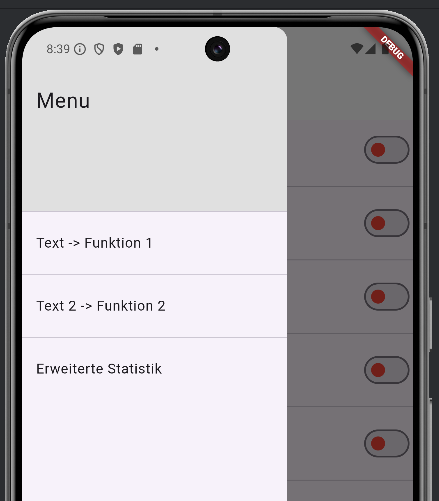
\includegraphics[height=4cm]{images/MenueScreen}
    \caption{Menüansicht, relevant ist die Funktion \enquote{Erweiterte Statistik}.}
\end{figure}

    \section{Gesamtstatistik.dart}
    Mit dem Aufruf der \enquote{Erweiterten Statistik} werden die Methoden der Datei \enquote{Gesamtstatistik.dart}
    getriggert. \\
    Zunächst erfolgt die Initialisierung einiger Variablen, die im weiteren Verlauf mit Werten befüllt und je nach
    Bedarf wieder geleert werden. \\
    Im weiteren Verlauf des Codes gibt es zudem mehrere Aufrufe an die Datei \enquote{postgresDatabase.dart},
    in der alle Datenbankabfragen gebündelt sind. \\
    Da wir eine eigene Datenbank erstellt haben, haben wir auch mit selbst definierten Dummydaten gearbeitet,
    die für uns realistisch Klangen und daher auch potenziell im Hauptsystem verwendet werden könnten.

    \begin{lstlisting}[language=Dart]
@override
Widget build(BuildContext context) {
  return Scaffold(
      appBar: AppBar(
        title: Text("Gesamtstatistik"),
 //...
        TextButton(
  onPressed: () async {
    setState(() {
      isYearly = true;
      _loadYearlyData();
    });
// ...
    ElevatedButton(
  onPressed: () {
    setState(() {
      isYearly = false;
      _loadDailyData();
    });
  },
// ...
      ),
  if (isYearly) _buildYearlyToggleButton(),
      Expanded(
    child: isYearly ? _buildYearlyView() : _buildDailyView(),
      ),
    ],
 // ...
}
    \end{lstlisting}
    Die \enquote{build()}-Methode ist dafür zuständig, die Seite der erweiterten Statistik initial zu laden.
    Zu Beginn wird standardmäßig die Jahresstatistik durch den Aufruf von \enquote{\_buildYearlyView()} dargestellt. \\
    Zusätzlich enthält die Methode zwei Buttons, mit denen der Nutzer zwischen der jährlichen, also \enquote{_buildYearlyView},
    und täglichen, \enquote{_buildDailyView}, Statistik wechseln kann.
    Je nach Auswahl werden die entsprechenden Bildschirme geladen und den damit verbundenen Statistikdaten.

    \begin{lstlisting}[language=Dart]
Future<void> _loadYearlyData() async {
    try {
        if (widget.database.connection.isClosed) {
        widget.database.connectToDatabase();
        }
        yearlyData = await widget.database.fetchYearlyStatistics();
        setState(() {});
    } catch (e) {
    print("Fehler beim Laden der Jahresdaten: $e");
    }
}
    \end{lstlisting}
    In dieser Methode wird zunächst überprüft, ob die Verbindung zur Datenbank noch aktiv ist.
    Da wir festgestellt haben, dass bei längerer Inaktivität der App die Verbindung automatisch getrennt wird. \\
    Falls die Verbindung geschlossen ist, wird sie mithilfe der bereits in der \enquote{main.dart} vorgestellten
    Methode erneut hergestellt.
    Ist die Verbindung noch aktiv, wird direkt mit dem Abruf der jährlichen Statistik fortgefahren.
    Nach dem erfolgreichen Abruf der Daten aus der Datenbank wird die Benutzeroberfläche mithilfe von
    \enquote{setState()} aktualisiert, sodass die neuen Daten unmittelbar im UI dargestellt werden.

    \begin{lstlisting}[language=Dart]
Future<List<Map<String, dynamic>>>
                    fetchYearlyStatistics() async {
  try {
    if(connection.isClosed) {
      connectWithRetry();
    }
    List<List<dynamic>> results = await connection.query('''
    SELECT
      jahr,
      COUNT(DISTINCT CASE WHEN batterie_status = 100 THEN DATE(
            jahr || '-' || monat || '-' || tag) END)
                                         AS anzahl_batterie_100,
      COUNT(DISTINCT CASE WHEN boiler_temp > 100 THEN DATE(
            jahr || '-' || monat || '-' || tag) END)
                                      AS anzahl_boiler_ueber_140
    FROM gesamtstatistik
    GROUP BY jahr
    ORDER BY jahr DESC;
    ''');

    return results.map((row) {
      return {
        'Jahr': row[0],
        'anzahl_batterie_100': row[1],
        'anzahl_boiler_ueber_140': row[2],
      };
    }).toList();
  } catch (e) {
    print('Fehler beim Abrufen der Jahresstatistik: $e');
    return [];
  }
}
    \end{lstlisting}
    Die Methode \enquote{fetchYearlyStatistics()} wird von \enquote{loadYearlyData()} aufgerufen und gehört zur Klasse
    \enquote{postgresDatabase}.
    Diese Trennung wurde bewusst vorgenommen, um alle Datenbankzugriffe in einer eigenen Klasse zu kapseln und
    den Code übersichtlicher zu gestalten.  \\
    Zu Beginn wird überprüft, ob eine Verbindung zur Datenbank aktiv ist.
    Falls die Verbindung geschlossen ist, wird die Methode \enquote{connectWithRetry()} aufgerufen, die eine Wiederherstellung der
    Verbindung mit Verzögerungen versucht.
    Nach erfolgreicher Verbindung wird eine SQL-Abfrage ausgeführt, deren Ergebnisse in einer dynamischen Liste
    gespeichert werden.
    Die Abfrage zählt die Anzahl der Tage pro Jahr, an denen:
    \begin{itemize}
        \item die Batterie einen Ladezustand von 100\% erreicht hat, und
        \item die Temperatur des Boilers 100 Grad überschritten hat.
    \end{itemize}
    Diese Selektion erfolgt durch die SQL-Funktion \enquote{COUNT(DISTINCT ...)}, die alle eindeutigen Tage zählt, an
    denen die jeweiligen Bedingungen erfüllt wurden.
    Diese Methode basiert auf dem Prinzip, welches wir in der Vorlesung \enquote{Datenbanken 1} gelernt haben.

    \begin{lstlisting}[language=Dart]
Widget _buildYearlyView() {
  return SingleChildScrollView(
    scrollDirection: Axis.horizontal,
    child: DataTable(
      columns: const [
        DataColumn(label: Text('Jahr')),
        DataColumn(label: Text('Batterie > 100%')),
        DataColumn(label: Text('Boiler > 100°C')),
      ],
      rows: yearlyData.map((data) {
        int year = data['Jahr'];
        int daysInYear = isLeapYear(year) ? 366 : 365;
        return DataRow(cells: [
          DataCell(Text('${data['Jahr']}')),
          DataCell(Text(showPercentage
              ? '${(data['anzahl_batterie_100'] / daysInYear * 100)
              .toStringAsFixed(2)}%'
              : '${data['anzahl_batterie_100']} / $daysInYear')),
          DataCell(Text(showPercentage
              ? '${(data['anzahl_boiler_ueber_140'] / daysInYear * 100)
              .toStringAsFixed(2)}%'
              : '${data['anzahl_boiler_ueber_140']} / $daysInYear')),
        ]);
      }).toList(),
    ),
  );
}
    \end{lstlisting}

    Die Methode \enquote{\_buildYearlyView()} holt die Werte aus der zuvor aufgerufenen Methode
    \enquote{\_loadYearlyData()} und verarbeitet diese zur Anzeige in einer \enquote{DataTable}.\\
    Die Tabelle besteht aktuell aus 3 Spalten und gibt die Anzahl an Tagen, in der sie ihre Abfrage erreicht hat.
    Die Werte für Batterie und Boiler können entweder \textbf{als absolute Anzahl der Tage oder als prozentualer Anteil}
    der gesamten Tage im jeweiligen Jahr angezeigt werden, welche durch \enqoute{showPercentage} gesteuert werden.
    Zusätzlich wird berücksichtigt, ob das Jahr ein Schaltjahr ist, da Schaltjahre 366 Tage haben, während normale Jahre 365 Tage umfassen.
    Diese Berechnung erfolgt mit der Methode \enquote{isLeapYear(year)}. \\
    Durch die Verwendung von \enquote{SingleChildScrollView} mit \enquote{Axis.horizontal} wird sichergestellt,
    dass die Tabelle scrollbar bleibt, falls die Inhalte über den verfügbaren Platz hinausgehen.

    \begin{lstlisting}[language=Dart]
Future<void> _loadDailyData() async {
  try {
    if (widget.database.connection.isClosed) {
      await widget.database.connectToDatabase();
    }
    if (fromDate != null && toDate != null) {
      dailyData = await widget.database.fetchDailyStatistics(
        startDate: fromDate,
        endDate: toDate,
      );
    } else if (fromDate != null && toDate == null) {
      dailyData = await widget.database.fetchDailyStatistics(
        startDate: fromDate,
      );
    } else if (fromDate == null && toDate != null){
      dailyData = await widget.database.fetchDailyStatistics(
        endDate: toDate,
      );
    } else {
      dailyData = await widget.database.fetchDailyStatistics();
    }
    setState(() {});
  } catch (e) {
    print("Fehler beim Laden der Tagesdaten: $e");
  }
}
    \end{lstlisting}
    Das Laden der täglichen Statistiken funktioniert grundsätzlich ähnlich wie bei der jährlichen Version.
    Der wesentliche Unterschied besteht jedoch darin, dass hier ein zusätzlicher Datumsfilter integriert wurde.
    Dieser Filter ermöglicht es, die Daten gezielt nach bestimmten Tagen oder Zeiträumen zu durchsuchen.
    Dadurch lassen sich einerseits unnötig große Datenmengen vermeiden und andererseits einzelne Tage gezielt analysieren.
    \begin{lstlisting}[language=Dart]
Future<List<Map<String, dynamic>>>
    fetchDailyStatistics({DateTime? startDate, DateTime? endDate}) async {
  try {
    if (connection.isClosed) {
      connectWithRetry();
    }
    String query = '''
    SELECT DISTINCT ON (Jahr, Monat, Tag)
      Jahr, Monat, Tag, MAX(batterie_status)
            AS batterie_status, MAX(boiler_temp) AS boiler_temp
    FROM gesamtstatistik
  ''';
    List<String> conditions = [];
    if (startDate != null && endDate != null) {
      conditions.add('Jahr >= ${startDate.year}
                                    AND Jahr <= ${endDate.year}');
      conditions.add('Monat >= ${startDate.month}
                                    AND Monat <= ${endDate.month}');
      conditions.add('Tag >= ${startDate.day}
                                    AND Tag <= ${endDate.day}');
    } else if (startDate != null && endDate == null) {
      conditions.add('Jahr >= ${startDate.year}');
      conditions.add('Monat >= ${startDate.month}');
      conditions.add('Tag >= ${startDate.day}');
    } else if (startDate == null && endDate != null) {
      conditions.add('Jahr <= ${endDate.year}');
      conditions.add('Monat <= ${endDate.month}');
      conditions.add('Tag <= ${endDate.day}');
    }
    if (conditions.isNotEmpty) {
      for(int i = 0; i < conditions.length; i++){
        if(i == 0){
          query += '\nWHERE ' + conditions.elementAt(i);
        } else {
          query += '\nAND ' + conditions.elementAt(i);
        }
      }
    }
    query += '\nGROUP BY Jahr, Monat, Tag\n
                    ORDER BY Jahr DESC, Monat DESC, Tag DESC';
    List<List<dynamic>> results = await connection.query(query);
    return results.map((row) {
      return {
        'Jahr': row[0],
        'Monat': row[1],
        'Tag': row[2],
        'batterie_status': row[3],
        'boiler_temp': row[4],
      };
    }).toList();
  } catch (e) {
    print('Fehler beim Abrufen der Tagesstatistik: $e');
    return [];
  }
}
    \end{lstlisting}
    In dieser Methode wird die SQL-Abfrage nicht direkt als fester String definiert, sondern als
    dynamischer String aufgebaut und während der Laufzeit ergänzt.
    Dies ermöglicht eine flexible Anpassung der Abfrage je nach den angegebenen Filterparametern.
    Mit der SQL-Funktion \enquote{MAX()} werden die höchsten Werte für \enquote{batterie\_status} und
    \enquote{boiler\_temp} pro Tag abgerufen.
    Durch die Kombination mit \enquote{GROUP BY Jahr, Monat, Tag} wird sichergestellt, dass die Werte für
    jeden einzelnen Tag separat aggregiert werden. \\
    Die Sortierung erfolgt mit \enquote{ORDER BY Jahr DESC, Monat DESC, Tag DESC}, sodass die neuesten
    Daten zuerst geladen und verarbeitet werden.
    Dadurch wird eine chronologisch absteigende Darstellung gewährleistet, bei der die aktuellsten
    Messwerte oben stehen und ältere Werte weiter unten folgen. \\
    Nach der finalen Zusammenstellung wird der SQL-String an die Datenbank gesendet.
    Die zurückgegebenen Ergebnisse werden in eine dynamische Liste umgewandelt, die dann weiterverarbeitet werden kann.
    Die beiden SQL-Abfragen sind recht flexibel und können mit kleineren Anpassungen mit anderen
    Tabellenstrukturen verwendet werden.
    \begin{lstlisting}[language=Dart]
Widget _buildDailyView() {
  final int pageCount = (dailyData.length / itemsPerPage).ceil();
  return Column(
    children: [
      _buildDateFilter(),
      if (dailyData.isEmpty)
        Expanded(
          child: Center(
            child: Text('Daten werden geladen.'),
          ),
        )
      else
      Expanded(
        child: Column(
        children: [
          Expanded(
            child: SingleChildScrollView(
              scrollDirection: Axis.vertical,
              child: SingleChildScrollView(
                scrollDirection: Axis.horizontal,
                child: DataTable(
                  columns: const [
                    DataColumn(label: Text('Datum')),
                    DataColumn(label: Text('Batterie = 100%')),
                    DataColumn(label: Text('Boiler > 100°C')),
                  ],
    // ...
    \end{lstlisting}
    Zunächst beginnt das Widget mit der Erstellung der und fragt ab, ob Daten überhaupt vorhanden sind, ist dies der Fall, wird ein Loading Screen imitiert,
    da wir sonst auf Fehler auf visuelle Fehler in der App kommen.
    Da alles Asynchron passiert wird währenddessen der Datumsfilter gebaut, welcher uns die einfache Möglichkeit erstellt,
    nach einem Datum zu sortieren.
    Im weiteren Verlauf wird die 3 Spaltenbreite Tabelle initialisiert.

    Das Widget \enquote{\_buildDailyView()} beginnt mit der Initialisierung und überprüft, ob Daten verfügbar sind.
    Falls keine Daten vorhanden sind, wird ein Ladebildschirm generiert. \\
    Dies verhindert visuelle Fehler in der App, die auftreten könnten, wenn versucht wird, nicht vorhandene Daten anzuzeigen.
    Da alle Prozesse asynchron ablaufen, wird währenddessen der Datumsfilter (\enquote{\_buildDateFilter()}) erstellt,
    um den User das Filtern nach Tag, Monat und Jahr zu ermöglichen.
    Um die Anzeige übersichtlich zu gestalten, wird in die Tabelle eine vertikalen und horizontalen
    Scroll-Funktion versehen, (\enquote{SingleChildScrollView}).
    \begin{lstlisting}[language=Dart]
      //...
child: DataTable (
    columns: const [
        DataColumn(label: Text('Datum')),
        DataColumn(label: Text('Batterie = 100\%')),
        DataColumn(label: Text('Boiler > 100C')),
    ],
  rows: dailyData
    .skip(currentPage * itemsPerPage)
    .take(itemsPerPage)
    .map((data) {
    bool batteryReached = double.parse(data['batterie_status']) == 100;
    bool boilerExceeded = (data['boiler_temp']) > 100;
    return DataRow(cells: [
      DataCell(Text('${data['Tag'].toString().padLeft(2, '0')}.
            ${data['Monat'].toString().padLeft(2, '0')}.${data['Jahr']}')),
      DataCell(Row(
        children: [
          batteryReached
            ? Icon(Icons.check, color: Colors.green) // Grüner Haken
            : Icon(Icons.close, color: Colors.red), // Rotes X
 // Pagination Steuerung
  Row(
    mainAxisAlignment: MainAxisAlignment.center,
        children: [
          IconButton(
            onPressed: currentPage > 0
            ? () {
              setState(() {
                currentPage--;
              });
            }
                : null,
            icon: Icon(Icons.arrow_back),
            ),
            Text('Seite ${currentPage + 1} von $pageCount'),
            IconButton(
            onPressed: currentPage < pageCount - 1
            ? () {
            setState(() {
                currentPage++;
            });
            }
    // ...
    }
    \end{lstlisting}
    Die Daten aus den Datenbankaufrufen werden aus DailyData entzogen und weiter verarbeitet. Sollte die Batterie an
    jenem Tag 100 Prozent erreicht haben oder der Boiler 100 Grad wird für diesen Tag ein Haken gesetzt,
    andernfalls ein rotes Kreuz. Weiters wurde mittels itemsperPage initialisiert wie viele Daten pro Seite
    angezeigt werden dürfen, um das Gerät zu entlasten und nicht tausende von Einträge zu haben.
    Initial wurde dies auf 40 Einträge pro Seite limitiert und durch die Länge der Liste und der Anzahl der Items werden
    die Anzahl der Seiten bestimmt. \\
    Weiter wurden Pfeile implementiert, die sog. IconButtons, welche durch die Seiten hin durch navigieren können.
    Die Daten aus den Datenbankabfragen werden aus \enquote{dailyData} entnommen und zur Anzeige weiterverarbeitet.
    Falls die Batterie an einem bestimmten Tag eine Ladung von \enquote{100\%} erreicht hat oder der Boiler eine
    Temperatur von über 100 Grad überschritten hat, wird für diesen Tag ein grüner Haken angezeigt.
    Andernfalls erscheint ein rotes Kreuz.

    \bibliography{main.bib}
    \bibliographystyle{plain}

\end{document}
